%%%%%%%%%%%%%%%%%%%%%%%%%%%%%%%%%%%%%%%%%%%%%%%%%%%%%%%%%%%%%%%%%%%%%%%%%%%%%%%%
%% Plantilla de memoria en LaTeX para la EIF - Universidad Rey Juan Carlos
%%
%% Por Gregorio Robles <grex arroba gsyc.urjc.es>
%%     Grupo de Sistemas y Comunicaciones
%%     Escuela de Ingeniería de Fuenlabrada
%%     Universidad Rey Juan Carlos
%% (muchas ideas tomadas de Internet, colegas del GSyC, antiguos alumnos...
%%  etc. Muchas gracias a todos)
%%
%% La última versión de esta plantilla está siempre disponible en:
%%     https://github.com/gregoriorobles/plantilla-memoria
%%
%% Para obtener PDF, ejecuta en la shell:
%%   make
%% (las imágenes deben ir en PNG o JPG)

%%%%%%%%%%%%%%%%%%%%%%%%%%%%%%%%%%%%%%%%%%%%%%%%%%%%%%%%%%%%%%%%%%%%%%%%%%%%%%%%

\documentclass[a4paper, 12pt]{book}
%\usepackage[T1]{fontenc}

\usepackage[a4paper, left=2.5cm, right=2.5cm, top=3cm, bottom=3cm]{geometry}
\usepackage{times}
\usepackage[utf8]{inputenc}
\usepackage[spanish]{babel} % Comenta esta línea si tu memoria es en inglés
\usepackage{url}
%\usepackage[dvipdfm]{graphicx}
\usepackage{graphicx}
\usepackage{float}  %% H para posicionar figuras
\usepackage[nottoc, notlot, notlof, notindex]{tocbibind} %% Opciones de índice
\usepackage{latexsym}  %% Logo LaTeX
\usepackage{tikz}

% Escribe el título y el nombre del autor / autora para que se use bien
% en otras partes de la plantilla
% Dependiendo de las partes de la plantilla, a veces aparecerán tal
% cual los escribas, a veces totalmente en mayúsculas, a veces de otras
% formas
\title{Título del Trabajo con Letras Mayúsculas para Sustantivos y Adjetivos}
\author{ José Matas Luque}

% Guarda el título, el autor y la fecha en variables
\makeatletter
\let\thetitle\@title
\let\theauthor\@author
\let\thedate\@date
\makeatother

\renewcommand{\baselinestretch}{1.5}  %% Interlineado

\begin{document}

\renewcommand{\refname}{Bibliografía}  %% Renombrando
\renewcommand{\appendixname}{Apéndice}


%%%%%%%%%%%%%%%%%%%%%%%%%%%%%%%%%%%%%%%%%%%%%%%%%%%%%%%%%%%%%%%%%%%%%%%%%%%%%%%%
% PORTADA

\begin{titlepage}
\begin{center}
\includegraphics[scale=0.6]{img/URJ_logo_Color_POS.png}

\vspace{1.75cm}

\LARGE
ESCUELA DE INGENIERÍA DE FUENLABRADA
\vspace{1cm}

\LARGE
TITULACIÓN EN MAYÚSCULAS

\vspace{1cm}
\LARGE
\textbf{TRABAJO FIN DE GRADO/MÁSTER}

\vspace{2cm}

\Large
\MakeUppercase{\thetitle}

\vspace{2cm}

\large
Autor : \theauthor \\
Tutor : Dr. Gregorio Robles\\
Cotutor: (si procede)
\vspace{1cm}

\large
Curso académico 2024/2025

\end{center}
\end{titlepage}

\newpage
\mbox{}
\thispagestyle{empty} % para que no se numere esta pagina



%%%%%%%%%%%%%%%%%%%%%%%%%%%%%%%%%%%%%%%%%%%%%%%%%%%%%%%%%%%%%%%%%%%%%%%%%%%%%%%%
%%%% Para firmar
\clearpage
\pagenumbering{gobble}
\chapter*{}

\vspace{-4cm}
\begin{center}
\LARGE
\textbf{Trabajo Fin de Grado}

\vspace{1cm}
\large
\thetitle

\vspace{0.8cm}
\large
\textbf{Autor :} \theauthor \\
\textbf{Tutor :} Dr. Nombre del Profesor/a

\end{center}

\vspace{0.8cm}
La defensa del presente Proyecto Fin de Carrera se realizó el día \qquad$\;\,$ de \qquad\qquad\qquad\qquad \newline de 2024, siendo calificada por el siguiente tribunal:


\vspace{0.5cm}
\textbf{Presidente:}

\vspace{1cm}
\textbf{Secretario:}

\vspace{1cm}
\textbf{Vocal:}


\vspace{1cm}
y habiendo obtenido la siguiente \textbf{Calificación:}


\vspace{1cm}
\begin{flushright}
Fuenlabrada, a \qquad$\;\,$ de \qquad\qquad\qquad\qquad de 202X
\end{flushright}

\vspace{1cm}

%% Licencia de publicación en abierto elegida
%% Ver detalles en https://ofilibre.urjc.es/guias/tfg-abierto/
\includegraphics[scale=0.6]{img/by-sa}
%\includegraphics[scale=0.6]{img/by}

%% Poner el año adecuado
\noindent©2024 \theauthor  \\
Algunos derechos reservados  \\
Este documento se distribuye bajo la licencia ``Atribución-CompartirIgual 4.0 Internacional'' de Creative Commons, disponible en \\
\url{https://creativecommons.org/licenses/by-sa/4.0/deed.es}


%%%%%%%%%%%%%%%%%%%%%%%%%%%%%%%%%%%%%%%%%%%%%%%%%%%%%%%%%%%%%%%%%%%%%%%%%%%%%%%%
%%%% Dedicatoria

\chapter*{}
\pagenumbering{Roman} % para comenzar la numeracion de paginas en numeros romanos
\begin{flushright}
\textit{Dedicado a \\
mi familia / mi abuelo / mi abuela}
\end{flushright}

%%%%%%%%%%%%%%%%%%%%%%%%%%%%%%%%%%%%%%%%%%%%%%%%%%%%%%%%%%%%%%%%%%%%%%%%%%%%%%%%
%%%% Agradecimientos

\chapter*{Agradecimientos}
%\addcontentsline{toc}{chapter}{Agradecimientos} % si queremos que aparezca en el índice
\markboth{AGRADECIMIENTOS}{AGRADECIMIENTOS} % encabezado 

Aquí vienen los agradecimientos\ldots Aunque está bien acordarse de la pareja, no hay que olvidarse de dar las gracias a tu madre, que aunque a veces no lo parezca disfrutará tanto de tus logros como tú\ldots 
Además, la pareja quizás no sea para siempre, pero tu madre sí.

%%%%%%%%%%%%%%%%%%%%%%%%%%%%%%%%%%%%%%%%%%%%%%%%%%%%%%%%%%%%%%%%%%%%%%%%%%%%%%%%
%%%% Resumen

\chapter*{Resumen}
%\addcontentsline{toc}{chapter}{Resumen} % si queremos que aparezca en el índice
\markboth{RESUMEN}{RESUMEN} % encabezado

Aquí viene un resumen del proyecto.
Ha de constar de tres o cuatro párrafos, donde se presente de manera clara y concisa de qué va el proyecto. 
Han de quedar respondidas las siguientes preguntas:

\begin{itemize}
  \item ¿De qué va este proyecto? ¿Cuál es su objetivo principal?
  \item ¿Cómo se ha realizado? ¿Qué tecnologías están involucradas?
  \item ¿En qué contexto se ha realizado el proyecto? ¿Es un proyecto dentro de un marco general?
\end{itemize}

Lo mejor es escribir el resumen al final.

%%%%%%%%%%%%%%%%%%%%%%%%%%%%%%%%%%%%%%%%%%%%%%%%%%%%%%%%%%%%%%%%%%%%%%%%%%%%%%%%
%%%% Resumen en inglés

\chapter*{Summary}
%\addcontentsline{toc}{chapter}{Summary} % si queremos que aparezca en el índice
\markboth{SUMMARY}{SUMMARY} % encabezado

Here comes a translation of the ``Resumen'' into English. 
Please, double check it for correct grammar and spelling.
As it is the translation of the ``Resumen'', which is supposed to be written at the end, this as well should be filled out just before submitting.


%%%%%%%%%%%%%%%%%%%%%%%%%%%%%%%%%%%%%%%%%%%%%%%%%%%%%%%%%%%%%%%%%%%%%%%%%%%%%%%%
%%%%%%%%%%%%%%%%%%%%%%%%%%%%%%%%%%%%%%%%%%%%%%%%%%%%%%%%%%%%%%%%%%%%%%%%%%%%%%%%
% ÍNDICES %
%%%%%%%%%%%%%%%%%%%%%%%%%%%%%%%%%%%%%%%%%%%%%%%%%%%%%%%%%%%%%%%%%%%%%%%%%%%%%%%%

% Las buenas noticias es que los índices se generan automáticamente.
% Lo único que tienes que hacer es elegir cuáles quieren que se generen,
% y comentar/descomentar esa instrucción de LaTeX.

%%%% Índice de contenidos
\tableofcontents 
%%%% Índice de figuras
\cleardoublepage
%\addcontentsline{toc}{chapter}{Lista de figuras} % para que aparezca en el indice de contenidos
\listoffigures % indice de figuras
%%%% Índice de tablas
%\cleardoublepage
%\addcontentsline{toc}{chapter}{Lista de tablas} % para que aparezca en el indice de contenidos
%\listoftables % indice de tablas


%%%%%%%%%%%%%%%%%%%%%%%%%%%%%%%%%%%%%%%%%%%%%%%%%%%%%%%%%%%%%%%%%%%%%%%%%%%%%%%%
%%%%%%%%%%%%%%%%%%%%%%%%%%%%%%%%%%%%%%%%%%%%%%%%%%%%%%%%%%%%%%%%%%%%%%%%%%%%%%%%
% INTRODUCCIÓN %
%%%%%%%%%%%%%%%%%%%%%%%%%%%%%%%%%%%%%%%%%%%%%%%%%%%%%%%%%%%%%%%%%%%%%%%%%%%%%%%%

\cleardoublepage
\chapter{Introducción}
\label{sec:intro} % etiqueta para poder referenciar luego en el texto con ~\ref{sec:intro}
\pagenumbering{arabic} % para empezar la numeración de página con números

% En este capítulo se introduce el proyecto.
% Debería tener información general sobre el mismo, dando la información sobre el contexto en el que se ha desarrollado.

% No te olvides de echarle un ojo a la página con los cinco errores de escritura más frecuentes\footnote{\url{http://www.tallerdeescritores.com/errores-de-escritura-frecuentes}}.

% Aconsejo a todo el mundo que mire y se inspire en memorias pasadas.
% Las memorias de los proyectos que he llevado yo están (casi) todas almacenadas en mi web del GSyC\footnote{\url{https://gsyc.urjc.es/~grex/pfcs/}}.

% En mayo de 2023 me apunté a un curso de innovación docente donde nos pidieron hacer un podcast con temática docente. Aproveché entonces para hacer un podcast de unos 30 minutos donde en los primeros quince minutos introducía LaTeX y la memoria, y en los segundos hacía hincapién en aquellas cosas que más os cuestan utilizar en la memoria: las figuras, las tablas y las citas. Podéis escuchar el podcast en Internet\footnote{\url{https://podcasters.spotify.com/pod/show/gregorio-robles9/episodes/Tu-memoria-de-Trabajo-Fin-de-Grado-o-de-Mster-en-LaTeX-e23hucr/a-a58kp2}}.


\section{Sección}
\label{sec:seccion}

Esto es una sección, que es una estructura menor que un capítulo. 

Por cierto, a veces me comentáis que no os compila por las tildes.
Eso es un problema de codificación.
Al guardar el archivo, guardad la codificación de ``ISO-Latin-1'' a ``UTF-8'' (o viceversa) y funcionará.

\section{Estilo}
\label{subsec:estilo}

Recomiendo leer los consejos prácticos sobre escribir documentos científicos en \LaTeX \ de Diomidis Spinellis\footnote{\url{https://github.com/dspinellis/latex-advice}}.

Lee sobre el uso de las comas\footnote{\url{http://narrativabreve.com/2015/02/opiniones-de-un-corrector-de-estilo-11-recetas-para-escribir-correctamente-la-coma.html}}. 
Las comas en español no se ponen al tuntún.
Y nunca, nunca entre el sujeto y el predicado (p.ej. en ``Yo, hago el TFG'' sobre la coma).
La coma no debe separar el sujeto del predicado en una oración, pues se cortaría la secuencia natural del discurso.
No se considera apropiado el uso de la llamada coma respiratoria o \emph{coma criminal}.
Solamente se suele escribir una coma para marcar el lugar que queda cuando omitimos el verbo de una oración, pero es un caso que se da de manera muy infrecuente al escribir un texto científico (p.ej. ``El Real Madrid, campeón de Europa'').

A continuación, viene una figura, la Figura~\ref{figura:foro_hilos}. 
Observarás que el texto dentro de la referencia es el identificador de la figura (que se corresponden con el ``label'' dentro de la misma). 
También habrás tomado nota de cómo se ponen las ``comillas dobles'' para que se muestren correctamente. 
Nota que hay unas comillas de inicio (``) y otras de cierre (''), y que son diferentes.
Volviendo a las referencias, nota que al compilar, la primera vez se crea un diccionario con las referencias, y en la segunda compilación se ``rellenan'' estas referencias. 
Por eso hay que compilar dos veces tu memoria.
Si no, no se crearán las referencias.



 \begin{figure}
    \centering
    \includegraphics[bb=0 0 800 600, width=12cm, keepaspectratio]{img/foro1}
    \caption{Página con enlaces a hilos}
    \label{figura:foro_hilos}
 \end{figure}


A continuación un bloque ``verbatim'', que se utiliza para mostrar texto tal cual.
Se puede utilizar para ofrecer el contenido de correos electrónicos, código, entre otras cosas.


{\footnotesize
\begin{verbatim}
    From gaurav at gold-solutions.co.uk  Fri Jan 14 14:51:11 2005
    From: gaurav at gold-solutions.co.uk (gaurav_gold)
    Date: Fri Jan 14 19:25:51 2005
    Subject: [Mailman-Users] mailman issues
    Message-ID: <003c01c4fa40$1d99b4c0$94592252@gaurav7klgnyif>

    Dear Sir/Madam,
    How can people reply to the mailing list?  How do i turn off
    this feature? How can i also enable a feature where if someone
    replies the newsletter the email gets deleted?
    Thanks

    From msapiro at value.net  Fri Jan 14 19:48:51 2005
    From: msapiro at value.net (Mark Sapiro)
    Date: Fri Jan 14 19:49:04 2005
    Subject: [Mailman-Users] mailman issues
    In-Reply-To: <003c01c4fa40$1d99b4c0$94592252@gaurav7klgnyif>
    Message-ID: <PC173020050114104851057801b04d55@msapiro>

    gaurav_gold wrote:
    >How can people reply to the mailing list?  How do i turn off
    this feature? How can i also enable a feature where if someone
    replies the newsletter the email gets deleted?

    See the FAQ
    >Mailman FAQ: http://www.python.org/cgi-bin/faqw-mm.py
    article 3.11
\end{verbatim}
}



\section{Estructura de la memoria}
\label{sec:estructura}


\begin{figure}
  \centering
  \includegraphics[width=9cm, keepaspectratio]{img/arquitectura.png}
  \caption{Estructura del parser básico}
  \label{fig:arquitectura}
\end{figure}




En esta sección se debería introducir la estructura de la memoria. 

Así:


\begin{itemize}
  \item En el primer capítulo se hace una intro al proyecto.
  
  \item En el capítulo~\ref{chap:objetivos} (ojo, otra referencia automática) se muestran los objetivos del proyecto.
  
  \item A continuación se presenta el estado del arte en el capítulo~\ref{chap:estado}.
  
  \item \ldots
\end{itemize}





%%%%%%%%%%%%%%%%%%%%%%%%%%%%%%%%%%%%%%%%%%%%%%%%%%%%%%%%%%%%%%%%%%%%%%%%%%%%%%%%
%%%%%%%%%%%%%%%%%%%%%%%%%%%%%%%%%%%%%%%%%%%%%%%%%%%%%%%%%%%%%%%%%%%%%%%%%%%%%%%%
% OBJETIVOS %
%%%%%%%%%%%%%%%%%%%%%%%%%%%%%%%%%%%%%%%%%%%%%%%%%%%%%%%%%%%%%%%%%%%%%%%%%%%%%%%%

\cleardoublepage % empezamos en página impar
\chapter{Objetivos} % título del capítulo (se muestra)
\label{chap:objetivos} % identificador del capítulo (no se muestra, es para poder referenciarlo)

\section{Objetivo general} % título de sección (se muestra)
\label{sec:objetivo-general} % identificador de sección (no se muestra, es para poder referenciarla)

% Aquí vendría el objetivo general en una frase:
% Mi trabajo fin de grado consiste en crear de una herramienta de análisis de los comentarios jocosos 
% en repositorios de software libre alojados en la plataforma GitHub.

% Recuerda que los objetivos siempre vienen en infinitivo.

El objetivo general del trabajo es realizar una revisión, reestructuración y extensión de funcionalidad del proyecto ya existente. Dicho proyecto se puede definir como una herramienta de análisis de código escrito en lenguaje Python.

\section{Objetivos específicos}
\label{sec:objetivos-especificos}

% Los objetivos específicos se pueden entender como las tareas en las que se ha desglosado el objetivo general.
% Y, sí, también vienen en infinitivo.

Los objetivos específicos de este trabajo se pueden definir de la siguiente manera:

\begin{itemize} 
    \item Optimizar el código existente para asegurar que el programa cumpla con los requisitos mínimos necesarios para su desarrollo futuro. 
    \item Implementar una funcionalidad de "plug-and-play" que permita a cualquier usuario descargar y utilizar el programa con una configuración mínima. 
    \item Incorporar un paquete de requisitos que incluya todas las dependencias y módulos necesarios para la correcta ejecución de la aplicación. 
    \item Mejorar la visualización de los resultados en formato JSON, facilitando su análisis posterior. 
    \item Desarrollar una interfaz web para la visualización de resultados, proporcionando una forma intuitiva de navegar entre los análisis realizados. 
    \item Implementar la visualización de resultados en la consola al finalizar el proceso de análisis. 
    \item Añadir registros detallados durante el proceso de análisis, para que el usuario pueda monitorizar el progreso y evitar la incertidumbre sobre el estado de ejecución en proyectos de larga duración. 
    \item  Reestructurar la arquitectura del código, reorganizando el árbol de directorios para asegurar una disposición lógica y coherente de los archivos, de acuerdo con los estándares recomendados en la industria. 
    \item Eliminar redundancias en el código e incorporar documentación detallada. 
    \item Ampliar el análisis con información adicional sobre el repositorio GitHub examinado, incluyendo datos relevantes sobre el autor y otros metadatos. \end{itemize}

\section{Planificación temporal}
\label{sec:planificacion-temporal}

% A mí me gusta que aquí pongáis una descripción de lo que os ha llevado realizar el trabajo.
% Hay gente que añade un diagrama de GANTT.
% Lo importante es que quede claro cuánto tiempo llevas (tiempo natural, p.ej., 6 meses) y a qué % nivel de esfuerzo (p.ej., principalmente los fines de semana).

El tiempo total asignado para el desarrollo del trabajo fue de seis meses. Durante los primeros meses, debido a compromisos laborales y las asignaturas del curso universitario, el tiempo disponible para dedicar al proyecto fue limitado, concentrándose principalmente en los fines de semana.

Dado que el proyecto se basa en la extensión de una aplicación preexistente, la primera fase consistió en comprender la estructura y funcionalidad del código ya implementado. Este proceso requirió más tiempo del estimado inicialmente, debido a la cantidad de errores, la falta de organización y la ausencia de documentación adecuada en el código existente.

Concluida esta fase de análisis, la primera tarea fue implementar la funcionalidad "plug-and-play". Sin embargo, este proceso se prolongó más de lo previsto debido a las dificultades para comprender el comportamiento del sistema durante la ejecución, ya que inicialmente presentaba fallos importantes que impedían su correcto funcionamiento.

Al finalizar el segundo mes de desarrollo, y tras haber establecido una base mínima operativa, pude realizar las primeras pruebas de ejecución, verificando los procesos a medida que los desarrollaba. Durante el tercer mes, me enfoqué en reescribir el código, eliminando una considerable cantidad de elementos redundantes, ineficientes e incluso obsoletos, garantizando además que tanto el código como la documentación cumplieran con los estándares de la industria.

Hacia mediados del cuarto mes, gran parte de la lógica de análisis ya había sido implementada. Aunque el desarrollo aún no estaba completamente finalizado, el progreso fue suficiente para iniciar pruebas del proceso en su totalidad, en lugar de continuar con las pruebas aisladas por partes realizadas previamente. A medida que comenzaba a obtener las primeras versiones de los resultados de los análisis, procedí a trabajar en la interfaz web y en la visualización de dichos resultados.

Durante el quinto mes, me enfoqué en finalizar la implementación del análisis y en realizar mejoras puntuales en diversas partes del proyecto que, aunque funcionales, podían optimizarse para mejorar tanto el rendimiento como la experiencia del usuario.

El sexto y último mes estuvo dedicado principalmente a la redacción de la memoria del proyecto. En cuanto al código, se realizaron ajustes menores para perfeccionar ciertos detalles, aunque ninguno de ellos representó un cambio significativo en el funcionamiento general del programa.





%%%%%%%%%%%%%%%%%%%%%%%%%%%%%%%%%%%%%%%%%%%%%%%%%%%%%%%%%%%%%%%%%%%%%%%%%%%%%%%%
%%%%%%%%%%%%%%%%%%%%%%%%%%%%%%%%%%%%%%%%%%%%%%%%%%%%%%%%%%%%%%%%%%%%%%%%%%%%%%%%
% ESTADO DEL ARTE %
%%%%%%%%%%%%%%%%%%%%%%%%%%%%%%%%%%%%%%%%%%%%%%%%%%%%%%%%%%%%%%%%%%%%%%%%%%%%%%%%

\cleardoublepage
\chapter{Estado del arte}
\label{chap:estado}

% Descripción de las tecnologías que utilizas en tu trabajo. 
% Con dos o tres párrafos por cada tecnología, vale. 
% Se supone que aquí viene todo lo que no has hecho tú.

% Puedes citar libros, como el de Bonabeau et al., sobre procesos 
% estigmérgicos~\cite{bonabeau:_swarm}. 
% Me encantan los procesos estigmérgicos.
% Deberías leer más sobre ellos.
% Pero quizás no ahora, que tenemos que terminar la memoria para sacarnos por fin el título.
% Nota que el \~ \ añade un espacio en blanco, pero no deja que exista un salto de línea. 
% Imprescindible ponerlo para las citas.

% Citar es importantísimo en textos científico-técnicos. 
% Porque no partimos de cero.
% Es más, partir de cero es de tontos; lo suyo es aprovecharse de lo ya existente para construir encima y hacer cosas más sofisticadas.
% ¿Dónde puedo encontrar textos científicos que referenciar?
% Un buen sitio es Google Scholar\footnote{\url{http://scholar.google.com}}.
% Por ejemplo, si buscas por ``stigmergy libre software'' para encontrar trabajo sobre software libre y el concepto de \emph{estigmergia} (¿te he comentado que me gusta el concepto de estigmergia ya?), encontrarás un artículo que escribí hace tiempo cuyo título es ``Self-organized development in libre software: a model based on the stigmergy concept''.
% Si pulsas sobre las comillas dobles (entre la estrella y el ``citado por ...'', justo debajo del extracto del resumen del artículo, te saldrá una ventana emergente con cómo citar.
% Abajo a la derecha, aparece un enlace BibTeX.
% Púlsalo y encontrarás la referencia en formato BibTeX, tal que así:

% {\footnotesize
% \begin{verbatim}
% @inproceedings{robles2005self,
 %  title={Self-organized development in libre software:
 %         a model based on the stigmergy concept},
%   author={Robles, Gregorio and Merelo, Juan Juli\'an 
 %          and Gonz\'alez-Barahona, Jes\'us M.},
 %  booktitle={ProSim'05},
%   year={2005}
% }
% \end{verbatim}
% }

% Copia el texto en BibTeX y pégalo en el fichero \texttt{memoria.bib}, que es donde están las referencias bibliográficas.
% Para incluir la referencia en el texto de la memoria, deberás citarlo, como hemos hecho antes con~\cite{bonabeau:_swarm}, lo que pasa es que en vez de el identificador de la cita anterior (bonabeau:\_swarm), tendrás que poner el nuevo (robles2005self).
% Compila el fichero \texttt{memoria.tex} (\texttt{pdflatex memoria.tex}), añade la bibliografía (\texttt{bibtex memoria.aux}) y vuelve a compilar \texttt{memoria.tex} (\texttt{pdflatex memoria.tex})\ldots y \emph{voilà} ¡tenemos una nueva cita~\cite{robles2005self}!

% También existe la posibilidad de poner notas al pie de página, por ejemplo, una para indicarte que visite la página del GSyC\footnote{\url{http://gsyc.es}}.

\section{Python}
Python es un lenguaje de programación de alto nivel ampliamente utilizado en el desarrollo de software. Es un lenguaje referente para tareas relacionadas con el análisis de datos y el auge de la IA ha aumentado aún más su popularidad. Su enfoque en la simplicidad y legibilidad del código, añadida a su gran polivalencia, lo convierte en una excelente opción para desarrolladores de todos los niveles.

Python es un lenguaje interpretado y de tipado dinámico, mas una de sus mayores virtudes es la presencia de una amplia biblioteca estándar y un ecosistema de paquetes más que robusto, el cual ofrece herramientas para prácticametne cualquier necesidad, desde desarrollo web hasta inteligencia artificial.

En el contexto de este proyecto Python ha sido utilizado como lenguaje principal para desarrollar la lógica del análisis, aprovechando su capacidad para manejar estructuras complejas de datos, así como su compatibilidad con bibliotecas de análisis, las cuales han sido cruciales para la tarea. La flexibilida del lenguaje ha permitido una rápida iteración y mejora del código, facilitanto también la integración con otras tecnologías.

\section{HTML}
HTML (HyperText Markup Language) es el lenguaje estándar para la creación y estructuración de documentos en la web. Define la estructura básica de las páginas web mediante el uso de etiquetas y atributos que organizan el contenido en elementos como encabezados, párrafos, listas, enlaces y multimedia. HTML proporciona la base sobre la cual se construyen las páginas web, permitiendo a los nevegadores interpretar y mostrar el contenido de manera coherente y estructurada.

En concreto, se utilizó HTML5, la versión más reciente del lenguaje, que introduce mejoras significativas con respecto a sus predecesores. HTML5 incluye nuevas etiquetas semánticas que mejoran la estructura del documento y la accesibilidad como \texttt{header}, \texttt{footer}, \texttt{article} y \texttt{section}. Estas etiquetas no sólo proporcional una estructura más clara y lógica para los documentos, sino que también facilitan la optimización para motores de búsqueda (SEO) y la integración con tecnlogías modernas. Además, HTML5 soporta de manera nativa elementos multimedia como <video> y <audio>, eliminando la hasta ahora necesaria incorporación de plugins adicionales y permitiendo una experiencia de usuario más rica y fluida.

En este proyecto HTML ha sido utilizado para construir y organizar la interfaz web, a fin de ofrecer una presentación moderna y funcional de los resultados del análisis.

\section{CSS}
CSS (Cascading Style Sheets) es el lenguaje utilizado para describir la presentación de un documento escrito en HTML. CSS permite la separación de la estructura de una página web de sus estilo visual, facilitando el mantenimiento y escalabilidad del diseño. Con CSS es posible definir elementos como colores, fuentes, espaciado y la disposición de los componentes de la página, logrando un diseño responsivo que se adapta a diferentes dispositivos y resoluciones de pantalla.

En este proyecto CSS ha sido empleado para mejorar la apariencia de la interfaz web, garantizando qeu los resultados visualizados fueran estéticamente atracticos y fáciles de interpretar. Además, CSS ha permitido personalizar el diseño para asegurar que la interfaz fuera todalmente responsiva, adptándose a dispotivos móviles y de escritorio sin pérdida de funcionalidad o usabilidad.

\section{JavaScript}
JavaScript es un lenguaje de programación orientado a eventos, utilizado principalmente para el desarrollo de la lógica en el lado del cliente en aplicaciones web, aunque no se limita únicamente a ese uso. Su capacidad para interactuar dinámicamente con el DOM (Document Object Model) lo convierte en el motor que ha impulsado durante décadas la interactividad de las páginas web modernas. A lo largo de los años, JavaScript ha evolucionado con frameworks y librerías que amplían sus funcionalidades y permiten el desarrollo de aplicaciones complejas tanto en el cliente como en el servidor.

En este proyecto, JavaScript se ha utilizado para diversos propósitos, incluyendo la implementación de funcionalidades en el servidor y en el cliente.

\begin{enumerate}
    \item \textbf{En el servidor:}
    \begin{itemize}
        \item \textbf{Manejo de rutas y archivos:} Se utiliza el framework Express.js para controlar el manejo de rutas y la creación de un servidor web. Express facilita la configuración de middleware para procesar solicitudes HTTP y servir archivos estáticos. En el código proporcionado, Express se usa para definir rutas que manejan solicitudes tanto para la API como para la entrega de archivos HTML y recursos estáticos, como imágenes, CSS y JavaScript.
        \item \textbf{Manejo de archivos:} Se utilizan módulos nativos de Node.js para leer y escribir archivos. En el código se leen archivos JSON y HTML y se ayuda a resolver rutas de archivos y directorios, asegurando la correcta ubicación de los archivos en el sistema de archivos.
        \item \textbf{API de resultados:} Se implementan rutas para servir resultados de análisis almacenados en archivos JSON. Esto incluye la lectura de directorios y el envío de datos JSON a través de una API RESTful, que permite que el cliente recupere información sobre los resultados de forma dinámica.
    \end{itemize}
    
    \item \textbf{En el cliente:}
    \begin{itemize}
        \item \textbf{Manipulación del DOM:} JavaScript se usa para modificar dinámicamente el contenido y estilo de la página web según los datos recibidos del servidor. Por ejemplo, se crean y actualizan elementos HTML, se gestionan tablas y se aplican estilos en función de las propiedades de los datos.
        \item \textbf{Interactividad:} Se implementan funcionalidades interactivas como la ordenación de tablas y la actualización dinámica de contenido. Las tablas se ordenan basándose en las interacciones del usuario y se ocultan o muestran elementos de la interfaz según el estado de los datos.
        \item \textbf{Llamadas a la API:} El código del cliente realiza solicitudes HTTP a la API del servidor. Los datos recuperados se utilizan para actualizar la interfaz de usuario, mostrando información relevante sobre los repositorios y sus resultados de análisis.
    \end{itemize}
\end{enumerate}

En resumen, JavaScript juega un papel crucial tanto en el lado del servidor como en el cliente en este proyecto. La integración con Express y la manipulación dinámica del DOM permiten una experiencia de usuario fluida y una interacción cómoda y eficiente con los datos almacenados. Esta combinación de tecnologías asegura que la aplicación web sea interactiva, receptiva y funcional, cumpliendo con los estándares modernos de desarrollo web.

\section{Node.js}
Node.js es un entorno de ejecución basado en el motor V8 de JavaScript, diseñado para ejecutar código JavaScript en el lado del servidor. Su principal fortaleza radica en su arquitectura de entrada/salida no bloqueante, lo que permite manejas múltiples conexiones de manera edificente. Esta característica lo convierte en una opción ideal para aplicaciones web en tiempo real y de alta concurrencia. Node.js ha ganado popularidad debido a su capacidad para crear aplicaciones escalables y su extenso ecosistema de paquetes, accesible a través de npm (Node Package Manager).

En este proyecto Node.js ha sido empleado como el entorno principal para el servidor frontend, permitiendo ejecutar el código de visualización de resultados y gestionar las interacciones con la interfaz web. Se utilizó para:

\begin{enumerate}
    \item \textbf{Ejecución de código de frontend:} Node.js ejecuta el código que gestiona la lógica del servidor, incluyendo la carga de archivos y la configuración de la API.
    \item \textbf{Interacción con Express.js:} Node.js permite la integración con Express.js para manejar las rutas y las solicitudes HTTP, ofreciente una plataforma robusta para el desarrollo del servidor.
    \item \textbf{Manejo de datos:} La arquitectura no bloqueante de Node.js es clave para manejar eficientemente grandes volúmenes de datos, optimizando el rendimiento del servidor.
\end{enumerate}

\section{Express}
Express es un framework web minimalista para Node.js, diseñado para crear aplicaciones web y APIs de manera sencilla y eficiente. Ofrece una estructura flexible y una serie de herramientas que permiten gestionar rutas, peticiones HTTP y middleware para agregar funcionalidades adicionales a una aplicación. Al ser ligero y altamente configurable Express es ideal para construir aplicaciones escalables y robustas en entornos de desarrollo modernos.

En el contexto de este proyecto Express ha sido fundamental para:

\begin{enumerate}
    \item \textbf{Definir rutas y middleware:} Express.js ha facilitado la configuración de rutas para manejar tanto la API como la entrega de recursos estáticos y dinámicos, permitiendo una correcta visualización de los resultados analizados.
    \item \textbf{Facilitar la comunicación cliente-servidor:} La integración de Express ha simplificado la gestión de las comunicaciones entre el cliente y el servidor, optimizando la entrega de datos y la actualización de la interfaz de usuario.
\end{enumerate}

\section{JSON}
JSON (JavaScript Object Notation) es un formato ligero de intercambio de datos que es fácil de leer y escribir para los humanos, y sencillo de interpretar y generar por las máquinas. Su estructura basada en pares clave-valor lo hace ideal para transportar datos entre un servidor y una aplicación web, o entre distintos componentes de un sistema distribuido. JSON es ampliamente utilizado en APIs y servicios web debido a su simplicidad y compatibilidad con mútliples lenguajes de programación.

En este proyecto JSON ha sido crucial en dos aspectos:

\begin{enumerate}
    \item \textbf{Almacenamiento de los resultados:} Los resultados del análisis se almacenan en archivos JSON. Este formato ha permitido una organización clara y estructurada de los datos, facilitando su prosterior manipulación y visualización.
    \item \textbf{Intercambio de datos con la API de GitHub:} La información devuelta por las llamadas HTTP a la API de GitHub también está en formato JSON. Esto ha permitido integrar de manera eficiente los datos externos en el sistema, asegurando una comunicación fluida entre las distintas partes del proyecto.
\end{enumerate}

La capacidad ed JSON para representar objetos de manera sencilla ha sido esencial para la eficiencia y flexibilidad del proyecto.

\section{VSCode}
Visual Studio Code (VSCode) es un editor de código fuente desarrollado por Microsoft en abril de 2015. Desde entonces ha sido ampliamente adoptado por la comunidad de desarrolladores debido a su ligereza y versatilidad.

VSCode ofrece una experiencia de desarrollo robusta con características como resaltado de sintaxis, autocompletado inteligente, plena integración con Git y una amplia selección de extensiones para mejor la productividad y añadir funcionalidades.

En este proyecto VSCode ha sido empleado como el entorno principal de desarrollo debido a sus numerosas ventajas:

\begin{enumerate}
    \item \textbf{Soporte para múltiples lenguajes: } A diferencia de otras herramientas VSCode tiene la capacidad de manejar tanto JavaScript, como Python y otros lenguajes clave del proyecto. Esta flexibilidad ha sido de vital importancia para facilitar el trabajo con el backend, frontend y la manipulación de datos.
    \item \textbf{Extensiones y depuracicón: } Se han utilizado extensiones específicas para los lenguajes empleados, lo que ha facilitado y acomodado el proceso de desarrollo.
    \item \textbf{Integración con Git: } La integración nativa de Git en VSCode ha permitido gestionar fácilmente el control de versiones del proyecto, permitiendo recuperar de manera sencilla trozos de código que han sido editados.
\end{enumerate}

En definitiva, la flexibilidad y ligereza de VSCode lo convierte en una herramienta esencial para el desarrollo ágil y eficiente del proyecto, ayudando a mantener un flujo de trabajo organizado y estable.

\section{Trello}
Trello es una herramienta de gestión de proyectos basada en el navegador que utiliza la metodología Kanban, la cual permite organizar tareas de forma visual e intuitiva mediante un sistema de tableros, listas y tarjetas. Los usuarios pueden mover tarjetas entre columnas para reflejar el estado de una tarea, facilitando la visualización del progreso de proyectos.

En este proyecto Trello ha sido utilizado para organizar las diferentes etapas de desarrollo, permitiendo mantener un registro de todas las tareas a realizar y el estado de las mismas. 

\section{Postman} Postman es una herramienta utilizada para probar y desarrollar APIs, que permite a los desarrolladores enviar peticiones HTTP a un servidor y verificar las respuestas de manera intuitiva. Su interfaz gráfica facilita la creación de peticiones \texttt{GET}, \texttt{POST}, \texttt{PUT}, \texttt{DELETE}, entre otras, y ofrece funcionalidades avanzadas como la creación de colecciones, pruebas automáticas y la posibilidad de compartir entornos de trabajo.

En el contexto de este proyecto Postman ha sido utilizado para:

\begin{enumerate}
    \item \textbf{Pruebas de APIs:} Se realizaron pruebas exhaustivas de las APIs desarrollados con Express y Node.js. Postman permitió verificar que las respuestas fueran correctas y que los datos se gestionaran adecuadamente en cada punto de la comunicación entre el cliente y el servidor.
    \item \textbf{Depuración y optimización:} La herramienta facilitó la identificación de errores y la optimización del rendimiento de las APIs. Su uso fue fundamental para asegurar la robustez y la funcionalidad de los endpoints antes de su implementación final.
\end{enumerate}

Postman ha sido de especial importancia para garantizar la calidad y fiabilidad del sistema al permitir una evaluación detallada de cada llamada HTTP realizada.

\label{sec:seccion1}

% Hemos hablado de cómo incluir figuras.
% Pero no hemos dicho nada de tablas.
% A mí me gustan las tablas.
% Mucho.
% Aquí un ejemplo de tabla, la Tabla~\ref{tab:ejemplo} (siento ser pesado, pero nota cómo he puesto la referencia).

% \begin{table}
 % \begin{center}
  % \begin{tabular}{ | l | c | r |} % tenemos tres colummnas, la primera alineada a la izquierda (l), la segunda al centro (c) y la tercera a la derecha (r). El | indica que entre las columnas habrá una línea separadora.
    % \hline
    % Uno & 2 & 3 \\ \hline % el hline nos da una línea vertical
    % Cuatro & 5 & 6 \\ \hline
    % Siete & 8 & 9 \\
    % \hline
  % \end{tabular}
  % \caption{Ejemplo de tabla. Aquí viene una pequeña descripción (el \emph{caption}, el pie de tabla/figura) del contenido de la tabla. Si la tabla no es autoexplicativa, siempre viene bien aclararla aquí.}
  % \label{tab:ejemplo}
 % \end{center}
% \end{table}

% Hay un sitio en Internet donde puedes diseñar las tablas fácilmente y luego hacer un corta y pega del resultado en tu editor.
% Puedes probarlo en \url{https://www.tablesgenerator.com/}.



%%%%%%%%%%%%%%%%%%%%%%%%%%%%%%%%%%%%%%%%%%%%%%%%%%%%%%%%%%%%%%%%%%%%%%%%%%%%%%%%
%%%%%%%%%%%%%%%%%%%%%%%%%%%%%%%%%%%%%%%%%%%%%%%%%%%%%%%%%%%%%%%%%%%%%%%%%%%%%%%%
% DISEÑO E IMPLEMENTACIÓN %
%%%%%%%%%%%%%%%%%%%%%%%%%%%%%%%%%%%%%%%%%%%%%%%%%%%%%%%%%%%%%%%%%%%%%%%%%%%%%%%%

\cleardoublepage
\chapter{Diseño e implementación}
\label{sec:diseno}

\section{Arquitectura general} 
\label{sec:arquitectura}

El objetivo de este proyecto es corregir y extender la funcionalidad, así como añadir una visualización web cómoda e intuitiva de los resultados obtenidos. Para ello hemos seguido los siguientes pasos:



\begin{figure}
  \centering
  \includegraphics[width=9cm, keepaspectratio]{img/arquitectura.png}
  \caption{Placeholder}
  \label{fig:arquitectura}
\end{figure}

\section{Obtención y comprensión del código existente}

El primer paso es muy básico pero indispensable. Debemos realizar una copia del repositorio original para obtener así un código del que partir que podamos modificar sin alterar el original. Una tarea no complicada que quedó solventada rápidamente mediante el uso de Git y Github. Hecho esto, podemos ponernos manos a la obra y comenzar a trabajar en el que a partir de ahora será nuestro código.

La mejor manera de comprender rápidamente qué haace un programa es ejecutándolo e ir, mediante ingeniería inversa, extrayendo qué está ocurriendo a medida que avanza la ejecución. Sin embargo, al intentar esto nos encontramos con que el programa presentaba una gran cantidad de errores y ni siquiera realizaba la labor que supuestamente debía. 

De este modo, hubo que virar el enfoque hacia una tarea diferente, volviéndose primordial el conseguir que el programa funcionase. Esto supuso un reto, porque en este punto todavía no estaba familiarizado con el código y desconocía qué debía hacer suponiendo que hiciese lo que debía, lo cual no era el caso.

\section{Creación de un registro de tareas}

El siguiente paso fue crear un nuevo tablero de Trello, del cual ya hemos hablado, para comenzar a recoger las tareas que iban apareciendo. Al principio del desarrollo estas tareas eran tan básicas como "Revisión y comprensión del código" y se volverían más específicas a medida que aumentara nuestro conocimiento sobre el proyecto.

Se realizaron diagramas de flujo para representar los proceso, con el fin de intentar entender y dejar anotado qué se realiza, dónde y cuándo.

\section{Solución de problemas de ejecución}

Comencé a editar pequeños fragmentos de código, a fin de intentar solucionar lo que pensaba en ese momento que eran los errores que impedían la correcta ejecución, pero a medida que unos se resolvían otros aparecían. Finalmente opté por rehacer el grueso del proyecto, dejando intacto de momento únicamente el proceso de análisis, es decir, la parte del programa que, dado cierto texto con código, lee y clasifica los elementos relacionados con Python que encuentra en el mismo.

De la parte del proyecto encargada se tomar y analizar los archivos sólo parecía funcionar (no daba error al instante) una de las 3 opciones, la de analizar un repositorio dado un enlace de GitHub. Las otras dos, analizar un usuario de Github y analizar un directorio local, las dejé temporalmente de lado para centrarme en la primera. Si lograba hacer funcionar una de ellas, las otras dos no debían ser muy diferentes.

Toda esta parte conforma lo que en el proyecto he denominado "backend", dando a entender que es el código encargado de hacer el procesamiento y cálculos necesarios para obtener los resultados. La otra gran parte del proyecto, el llamado "frontend", sufría el mismo problema y daba errores de ejecución. De nuevo opté por rehacer el archivo principal que manejaba esa parte, obteniendo así unas primeras versiones ejecutables del código.

\section{Reestructuración y mejoras preparativas}

Una vez establecida una base ejecutable realicé unas últimas revisiones al código para asegurar el entendimiento del mismo. Además, antes de comenzar a implementar las nuevas funcionalidades se realizaron múltiples mejoras para facilitar el trabajo futuro:

\begin{itemize}
    \item Renombramiento y reelaboración de funciones para adecuarse a los estándares y simplificar su edición a futuros usuarios, utilizando nombres más representativos que expliquen rápidamente su finalidad.
    \item Añadida documentación.
    \item Reestructuración general del proyecto, diferenciando el código de backend y frontend en sus respectivas carpetas.
    \item Añadidos archivos de requisitos que el usuario puede utilizar para instalar rápidamente todo lo necesario para ejecutar el proyecto.
    \item Añadidos logs para que el usuario sepa en todo momento qué está realizando el programa. La demora del análisis en proyectos de gran tamaño pueden dar a entender al usuario que se ha parado cuando no es así. Estos logs vienen acompañados de mensajes de error descriptivos que indican al usuario por qué ha fallado el programa en caso de hacerlo.
\end{itemize}

\section{Implementación de nuevas funcionalidades}

Establecidas estas mejoras podemos comenzar a implementar desarrollos que extiendan las funcionalidades del proyecto actual. Puesto que el proyecto consta de dos grandes ramas, las agruperos de acorde a cuál de éstas pertenecen:

\subsection{Backend}

En lo relativo al backend encontramos la parte del proyecto encargada de procesar el input del usuario con el fin de recabar los datos necesarios y realizar el análisis que convenga. Los cambios más relevantes en esta parte son los siguientes:

\begin{itemize}
    \item \textbf{Extensión del análisis del repositorio }, incluyendo información relevante sobre el historial del mismo y de los usuarios que han participado en él. En caso de analizar un directorio local el programa comprobará antes si forma parte de un repositorio en Github. En caso de ser así, preguntará al usuario si prefiere analizar directamente el repositorio en cuestión en lugar de los archivos locales. Las ventajas que tiene esto son (1) el directorio local puede no estar actualizado con los últimos cambios subidos al repositorio, de modo que al analizar directamente la versión de GitHub nos aseguramos de estar analizando la última versión compartida, y (2) nos añade a los resultados del análisis esa información referente a GitHub, en lugar de únicamente la del código.

    \item \textbf{Mejora del archivo resultante del análisis} para facilitar su posterior tratamiento. Originalmente se generaban dos archivos equivalentes en formatos JSON y CSV. Aunque ambos formatos son ampliamente utilizados para el análisis de datos, hemos optado por mantener únicamente el formato JSON debido a su mayor flexibilidad para estructurar y manipular información. A diferencia del CSV, que se ajusta mejor a datos tabulares con campos claramente definidos y fijos, el JSON permite cambios más dinámicos en la estructura de los datos sin la necesidad de realizar ajustes constantes para que los campos se adapten a un formato rígido. Esto hace que el JSON sea más adecuado para futuras reestructuraciones del archivo, evitando la complejidad asociada a modificar archivos CSV cuando la estructura de los datos cambia significativamente. Al prescindir del archivo CSV, simplificamos el proceso de manejo y actualización de los datos, permitiendo una mayor versatilidad en su tratamiento y reduciendo las dificultades asociadas al ajuste de formatos estáticos como el CSV.

    \item \textbf{Añadida visualización de resultados desde la terminal}, en caso de que el usuario prefiera una vista rápida de los resultados sin tener que depender de la parte web. 

\begin{figure}
  \centering
  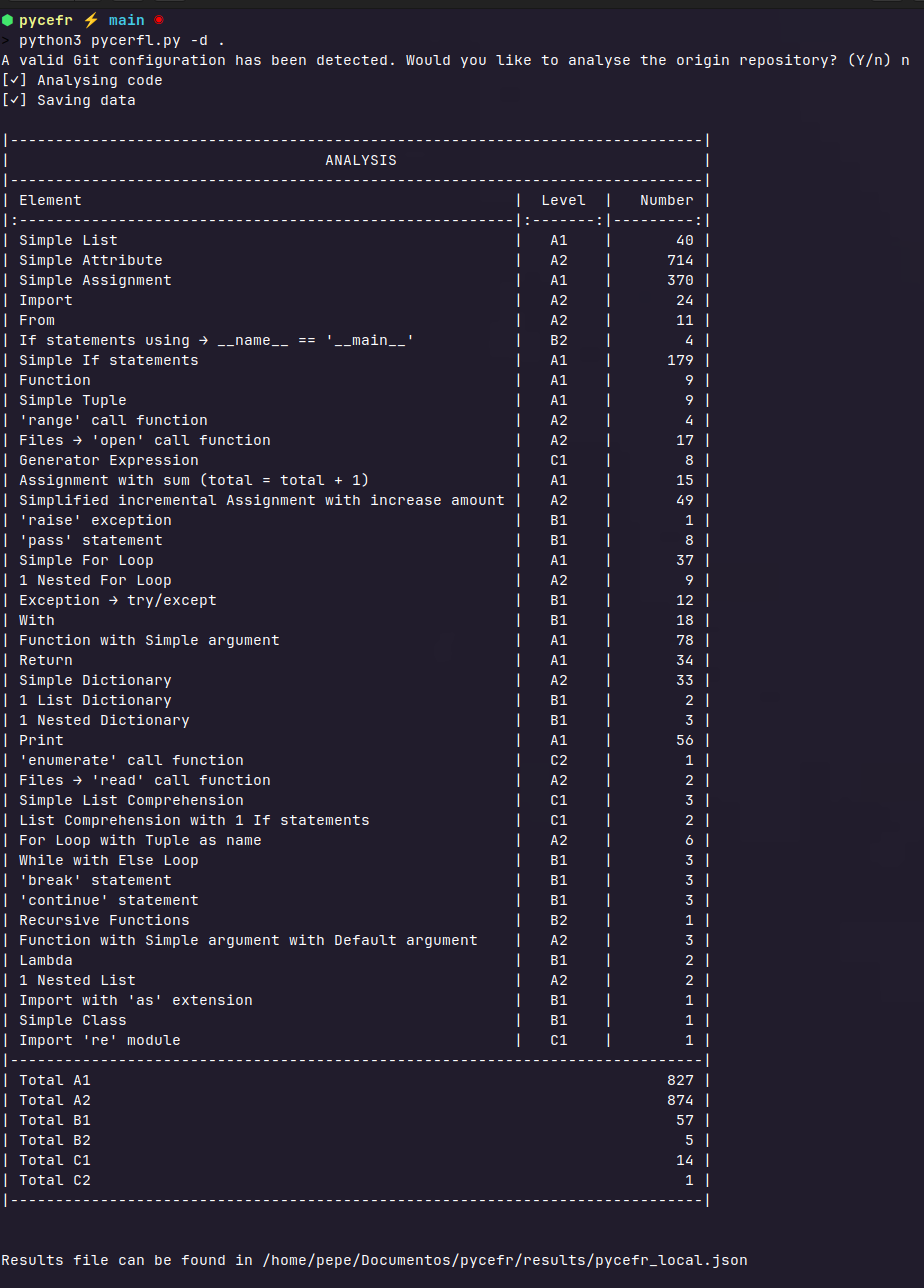
\includegraphics[width=14cm, keepaspectratio]{img/execution_local.png}
  \caption{Vista de resultados por consola tras análisis de directorio local}
  \label{fig:execution_local}
\end{figure}
    
\end{itemize}

\subsection{Frontend}

Utilizamos el término "frontend" para la parte del proyecto encargada de la web. En nuestro caso usamos la web para la navegación y visualización de los archivos producidos como resultado de los análisis.

La versión original del frontend es funcional, en el sentido de que cumple su labor, pero presentaba una estructura muy básica y poco modular. Todo el código estaba contenido en un único archivo `main.js`, que generaba dinámicamente un archivo HTML e insertaba directamente toda la información en la página. Esto no solo dificultaba la escalabilidad del proyecto, sino que también limitaba la separación de responsabilidades entre las diferentes partes del frontend y hacía más complicado el mantenimiento del código a largo plazo.

En el rediseño completo del frontend, hemos implementado una estructura más profesional y escalable. Se han organizado los recursos del proyecto en carpetas separadas, como `public`, `assets`, `html`, `css` y `js`, siguiendo las buenas prácticas del desarrollo web moderno. Asimismo, se ha incluido un archivo `package.json`, fundamental para gestionar las dependencias del proyecto y definir los scripts necesarios para su ejecución. El uso de `npm` como gestor de dependencias permite que el proyecto sea fácilmente reproducible en cualquier entorno, garantizando que todas las bibliotecas y módulos requeridos puedan ser instalados de manera automática y coherente.

Para el servidor, hemos adoptado `Express.js` como framework, creando un archivo `server.js` dedicado a cargar y gestionar el servidor web, lo que no existía en la versión anterior. También se han implementado rutas específicas para la API (`apiRoutes.js`) y para servir las páginas HTML (`htmlRoutes.js`), lo que proporciona una clara separación entre la lógica de backend y la presentación de los datos. Esto mejora el manejo de peticiones y la organización del código, haciendo más eficiente la gestión del servidor y la comunicación entre las distintas capas de la aplicación.

Además, el uso del `package.json` facilita la futura definición de scripts para tareas comunes como la ejecución del servidor en modo desarrollo, la instalación de dependencias y el despliegue. Esto asegura que todos los colaboradores del proyecto puedan utilizar los mismos comandos y configuraciones, evitando problemas derivados de configuraciones locales.

En resumen, este rediseño transforma el frontend en un proyecto más modular, mantenible y alineado con estándares profesionales, lo que facilita tanto su evolución futura como la colaboración en equipo. La inclusión de `Express.js`, junto con el uso de `npm` y un `package.json` bien definido, asegura que la gestión de dependencias y la ejecución del proyecto sean eficientes y consistentes.

En la siguiente comparativa se puede observar el cambio significativo en la estructura del frontend tras el rediseño. La imagen de la izquierda muestra el árbol de archivos original, donde todo el código estaba contenido en un único archivo `main.js`. Por el contrario, la imagen de la derecha ilustra el nuevo diseño, que adopta una estructura modular y organizada en carpetas, incluyendo archivos específicos para las rutas de la API, los estilos, los scripts, y el uso de `Express.js` para la gestión del servidor.


\vspace{2em}
\begin{figure}[htbp]
  \centering
  \begin{minipage}[t]{0.35\textwidth}
    \centering
    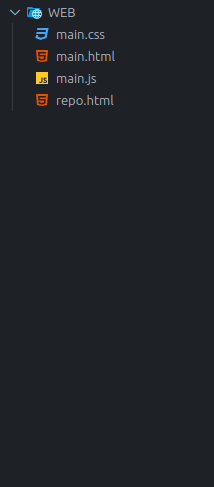
\includegraphics[width=\textwidth, keepaspectratio]{img/tree_frontend_original.png}
    \caption{Estructura original del frontend}
    \label{fig:original_structure}
  \end{minipage}
  \hspace{0.1\textwidth}
  \begin{minipage}[t]{0.35\textwidth}
    \centering
    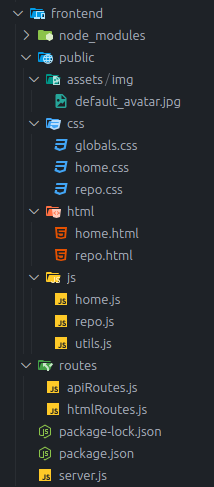
\includegraphics[width=\textwidth, keepaspectratio]{img/tree_frontend_final.png}
    \caption{Nueva estructura del frontend tras el rediseño}
    \label{fig:new_structure}
  \end{minipage}
\end{figure}



%Por ejemplo, puedes verlo en la figura~\ref{fig:arquitectura}.
%\LaTeX \ pone las figuras donde mejor cuadran. 
%Y eso quiere decir que quizás no lo haga donde lo hemos puesto\ldots 
%Eso no es malo.
%A veces queda un poco raro, pero es la filosofía de \LaTeX: tú al contenido, que yo me encargo de la maquetación.


 
%Recuerda que toda figura que añadas a tu memoria debe ser explicada.
%Sí, aunque te parezca evidente lo que se ve en la figura~\ref{fig:arquitectura}, la figura en sí solamente es un apoyo a tu texto.
%Así que explica lo que se ve en la figura, haciendo referencia a la misma tal y como ves aquí.
%Por ejemplo: En la figura~\ref{fig:arquitectura} se puede ver que la estructura del \emph{parser} básico, que consta de seis componentes diferentes: los datos se obtienen de la red, y según el tipo de dato, se pasará a un \emph{parser} específico y bla, bla, bla\ldots

% Si utilizas una base de datos, no te olvides de incluir también un diagrama de entidad-relación.


%%%%%%%%%%%%%%%%%%%%%%%%%%%%%%%%%%%%%%%%%%%%%%%%%%%%%%%%%%%%%%%%%%%%%%%%%%%%%%%%
%%%%%%%%%%%%%%%%%%%%%%%%%%%%%%%%%%%%%%%%%%%%%%%%%%%%%%%%%%%%%%%%%%%%%%%%%%%%%%%%
% EXPERIMENTOS Y VALIDACIÓN %
%%%%%%%%%%%%%%%%%%%%%%%%%%%%%%%%%%%%%%%%%%%%%%%%%%%%%%%%%%%%%%%%%%%%%%%%%%%%%%%%

\cleardoublepage
\chapter{Experimentos y validación}
\label{chap:experimentos}

Este capítulo se introdujo como requisito en 2019. 
Describe los experimentos y casos de test que tuviste que implementar para validar tus resultados. 
Incluye también los resultados de validación que permiten afirmar que tus resultados son correctos. 


%%%%%%%%%%%%%%%%%%%%%%%%%%%%%%%%%%%%%%%%%%%%%%%%%%%%%%%%%%%%%%%%%%%%%%%%%%%%%%%%
%%%%%%%%%%%%%%%%%%%%%%%%%%%%%%%%%%%%%%%%%%%%%%%%%%%%%%%%%%%%%%%%%%%%%%%%%%%%%%%%
% RESULTADOS %
%%%%%%%%%%%%%%%%%%%%%%%%%%%%%%%%%%%%%%%%%%%%%%%%%%%%%%%%%%%%%%%%%%%%%%%%%%%%%%%%

\cleardoublepage
\chapter{Resultados}
\label{chap:resultados}

En este capítulo se incluyen los resultados de tu trabajo fin de grado.

Si es una herramienta de análisis lo que has realizado, aquí puedes poner ejemplos de haberla utilizado para que se vea su utilidad.


%%%%%%%%%%%%%%%%%%%%%%%%%%%%%%%%%%%%%%%%%%%%%%%%%%%%%%%%%%%%%%%%%%%%%%%%%%%%%%%%
%%%%%%%%%%%%%%%%%%%%%%%%%%%%%%%%%%%%%%%%%%%%%%%%%%%%%%%%%%%%%%%%%%%%%%%%%%%%%%%%
% CONCLUSIONES %
%%%%%%%%%%%%%%%%%%%%%%%%%%%%%%%%%%%%%%%%%%%%%%%%%%%%%%%%%%%%%%%%%%%%%%%%%%%%%%%%

\cleardoublepage
\chapter{Conclusiones}
\label{chap:conclusiones}


\section{Consecución de objetivos}
\label{sec:consecucion-objetivos}

Esta sección es la sección espejo de las dos primeras del capítulo de objetivos, donde se planteaba el objetivo general y se elaboraban los específicos.

Es aquí donde hay que debatir qué se ha conseguido y qué no. 
Cuando algo no se ha conseguido, se ha de justificar, en términos de qué problemas se han encontrado y qué medidas se han tomado para mitigar esos problemas.

Y si has llegado hasta aquí, siempre es bueno pasarle el corrector ortográfico, que las erratas quedan fatal en la memoria final.
Para eso, en Linux tenemos aspell, que se ejecuta de la siguiente manera desde la línea de \emph{shell}:

\begin{verbatim}
  aspell --lang=es_ES -c memoria.tex
\end{verbatim}

\section{Aplicación de lo aprendido}
\label{sec:aplicacion}

Aquí viene lo que has aprendido durante el Grado/Máster y que has aplicado en el TFG/TFM.
Una buena idea es poner las asignaturas más relacionadas y comentar en un párrafo los conocimientos y habilidades puestos en práctica.

\begin{enumerate}
  \item a
  \item b
\end{enumerate}


\section{Lecciones aprendidas}
\label{sec:lecciones_aprendidas}

Aquí viene lo que has aprendido en el Trabajo Fin de Grado/Máster.

\begin{enumerate}
  \item Aquí viene uno.
  \item Aquí viene otro.
\end{enumerate}


\section{Trabajos futuros}
\label{sec:trabajos_futuros}

Ningún proyecto ni software se termina, así que aquí vienen ideas y funcionalidades que estaría bien tener implementadas en el futuro.

Es un apartado que sirve para dar ideas de cara a futuros TFGs/TFMs.


%%%%%%%%%%%%%%%%%%%%%%%%%%%%%%%%%%%%%%%%%%%%%%%%%%%%%%%%%%%%%%%%%%%%%%%%%%%%%%%%
%%%%%%%%%%%%%%%%%%%%%%%%%%%%%%%%%%%%%%%%%%%%%%%%%%%%%%%%%%%%%%%%%%%%%%%%%%%%%%%%
% APÉNDICE(S) %
%%%%%%%%%%%%%%%%%%%%%%%%%%%%%%%%%%%%%%%%%%%%%%%%%%%%%%%%%%%%%%%%%%%%%%%%%%%%%%%%

\cleardoublepage
\appendix
\chapter{Manual de usuario}
\label{app:manual}

Esto es un apéndice.
Si has creado una aplicación, siempre viene bien tener un manual de usuario.
Pues ponlo aquí.

%%%%%%%%%%%%%%%%%%%%%%%%%%%%%%%%%%%%%%%%%%%%%%%%%%%%%%%%%%%%%%%%%%%%%%%%%%%%%%%%
%%%%%%%%%%%%%%%%%%%%%%%%%%%%%%%%%%%%%%%%%%%%%%%%%%%%%%%%%%%%%%%%%%%%%%%%%%%%%%%%
% BIBLIOGRAFIA %
%%%%%%%%%%%%%%%%%%%%%%%%%%%%%%%%%%%%%%%%%%%%%%%%%%%%%%%%%%%%%%%%%%%%%%%%%%%%%%%%

\cleardoublepage

% Las siguientes dos instrucciones es todo lo que necesitas
% para incluir las citas en la memoria
\bibliographystyle{abbrv}
\bibliography{memoria}  % memoria.bib es el nombre del fichero que contiene
% las referencias bibliográficas. Abre ese fichero y mira el formato que tiene,
% que se conoce como BibTeX. Hay muchos sitios que exportan referencias en
% formato BibTeX. Prueba a buscar en http://scholar.google.com por referencias
% y verás que lo puedes hacer de manera sencilla.
% Más información: 
% http://texblog.org/2014/04/22/using-google-scholar-to-download-bibtex-citations/

\end{document}
